
%%%%%%%%%%%%%%%%%%%%%%%%%%%%%%%%%%%%%%%%%
% Structured General Purpose Assignment
% LaTeX Template
%
% This template has been downloaded from:
% http://www.latextemplates.com
%
% Original author:
% Ted Pavlic (http://www.tedpavlic.com)
%
% Note:
% The \lipsum[#] commands throughout this template generate dummy text
% to fill the template out. These commands should all be removed when 
% writing assignment content.
%
%%%%%%%%%%%%%%%%%%%%%%%%%%%%%%%%%%%%%%%%%

%----------------------------------------------------------------------------------------
%	PACKAGES AND OTHER DOCUMENT CONFIGURATIONS
%----------------------------------------------------------------------------------------

\documentclass{article}

\usepackage{fancyhdr} % Required for custom headers
\usepackage{lastpage} % Required to determine the last page for the footer
\usepackage{extramarks} % Required for headers and footers
\usepackage{graphicx} % Required to insert images
\usepackage{lipsum} % Used for inserting dummy 'Lorem ipsum' text into the template

% Margins
\topmargin=-0.45in
\evensidemargin=0in
\oddsidemargin=0in
\textwidth=6.5in
\textheight=9.0in
\headsep=0.25in 

\linespread{1.1} % Line spacing
\pdfinfo{
   /Author (Sainyam Kapoor)
   /Title  (Assignment)
   /CreationDate (D:20140115195600)
   /Subject (Assignment1)
   /Keywords (PDF;assignment CS-2202)
}
% Set up the header and footer
\pagestyle{fancy}
\lhead{\hmwkAuthorName} % Top left header
\chead{\hmwkClass\ (\hmwkClassInstructor\ ): \hmwkTitle} % Top center header
\rhead{\firstxmark} % Top right header
\lfoot{\lastxmark} % Bottom left footer
\cfoot{} % Bottom center footer
\rfoot{Page\ \thepage\ of\ \pageref{LastPage}} % Bottom right footer
\renewcommand\headrulewidth{0.4pt} % Size of the header rule
\renewcommand\footrulewidth{0.4pt} % Size of the footer rule

\setlength\parindent{0pt} % Removes all indentation from paragraphs

%----------------------------------------------------------------------------------------
%	DOCUMENT STRUCTURE COMMANDS
%	Skip this unless you know what you're doing
%----------------------------------------------------------------------------------------

% Header and footer for when a page split occurs within a problem environment
\newcommand{\enterProblemHeader}[1]{
\nobreak\extramarks{#1}{#1 continued on next page\ldots}\nobreak
\nobreak\extramarks{#1 (continued)}{#1 continued on next page\ldots}\nobreak
}

% Header and footer for when a page split occurs between problem environments
\newcommand{\exitProblemHeader}[1]{
\nobreak\extramarks{#1 (continued)}{#1 continued on next page\ldots}\nobreak
\nobreak\extramarks{#1}{}\nobreak
}

\setcounter{secnumdepth}{0} % Removes default section numbers
\newcounter{homeworkProblemCounter} % Creates a counter to keep track of the number of problems

\newcommand{\homeworkProblemName}{}
\newenvironment{homeworkProblem}[1][Problem \arabic{homeworkProblemCounter}]{ % Makes a new environment called homeworkProblem which takes 1 argument (custom name) but the default is "Problem #"
\stepcounter{homeworkProblemCounter} % Increase counter for number of problems
\renewcommand{\homeworkProblemName}{#1} % Assign \homeworkProblemName the name of the problem
\section{\homeworkProblemName} % Make a section in the document with the custom problem count
\enterProblemHeader{\homeworkProblemName} % Header and footer within the environment
}{
\exitProblemHeader{\homeworkProblemName} % Header and footer after the environment
}

\newcommand{\problemAnswer}[1]{ % Defines the problem answer command with the content as the only argument
\noindent\framebox[\columnwidth][c]{\begin{minipage}{0.98\columnwidth}#1\end{minipage}} % Makes the box around the problem answer and puts the content inside
}

\newcommand{\homeworkSectionName}{}
\newenvironment{homeworkSection}[1]{ % New environment for sections within homework problems, takes 1 argument - the name of the section
\renewcommand{\homeworkSectionName}{#1} % Assign \homeworkSectionName to the name of the section from the environment argument
\subsection{\homeworkSectionName} % Make a subsection with the custom name of the subsection
\enterProblemHeader{\homeworkProblemName\ [\homeworkSectionName]} % Header and footer within the environment
}{
\enterProblemHeader{\homeworkProblemName} % Header and footer after the environment
}
   
%----------------------------------------------------------------------------------------
%	NAME AND CLASS SECTION
%----------------------------------------------------------------------------------------

\newcommand{\hmwkTitle}{Assignment\ \#1} % Assignment title
\newcommand{\hmwkDueDate}{Saturday,\ January\ 25,\ 2014} % Due date
\newcommand{\hmwkClass}{CS-2202} 
\newcommand{\hmwkClassName}{DIGITAL CKTS. AND LOGIC DESIGN} % Course/class

\newcommand{\hmwkClassInstructor}{Dr. Ravi Shankar Singh} % Teacher/lecturer
\newcommand{\hmwkAuthorName}{Sainyam Kapoor} % Your name

%----------------------------------------------------------------------------------------
%	TITLE PAGE
%----------------------------------------------------------------------------------------

\title{
\vspace{2in}
\textmd{\textbf{\hmwkClass:\ \hmwkTitle\\~\\ \hmwkClassName}}\\
\normalsize\vspace{0.1in}\small{Due\ on\ \hmwkDueDate}\\
\vspace{0.1in}\large{\textit{Submitted to \hmwkClassInstructor\ }}
\vspace{2in}
\vspace{0.1in}\large{\textit{\\~\\Submitted by }}}

\author
 {
\textbf{\hmwkAuthorName}
\\~\\
\textit{12400EN003}
}

\date{23 January 2014} % Insert date here if you want it to appear below your name

%----------------------------------------------------------------------------------------

\begin{document}

\maketitle

\clearpage

%----------------------------------------------------------------------------------------
%	PROBLEM 1
%----------------------------------------------------------------------------------------

% To have just one problem per page, simply put a \clearpage after each problem

\begin{homeworkProblem}
\textbf{Draw a full adder using two half adders and one OR gate only.} \vspace{10pt} % Question

\problemAnswer{ 

Following is the circuit diagram for a full adder constructed using 2 half adders and one OR gate. Three numbers can be added as follows \\~\\
P+Q+C = (P+Q) + C. 

\begin{center}
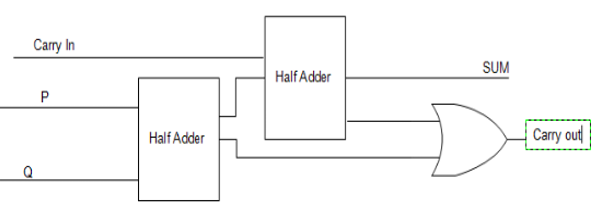
\includegraphics[width=0.75\columnwidth]{q1} % Example image
\end{center}
Now P + Q can be calculated using half adder and the sum of the first 2 numbers can be given as input to the next half adder. For the carry to be one only 2 cases are possible \\~\\Case 1: P + Q = 2 \\~\\ Case 2: P + Q = 1 and C = 1.\\~\\Thus the carry given by the full adder will be the logical or of the carry given by the 2 half adders.}
\end{homeworkProblem}

%----------------------------------------------------------------------------------------
%	PROBLEM 1
%----------------------------------------------------------------------------------------

% To have just one problem per page, simply put a \clearpage after each problem
\clearpage
\begin{homeworkProblem}
\textbf{Draw a full subtractor using two half subtractors and one OR gate only.}  \vspace{10pt} % Question

\problemAnswer{ 

Following is a Full subtractor implemented through the use if 2 half subtractors and one OR gate.
\begin{center}
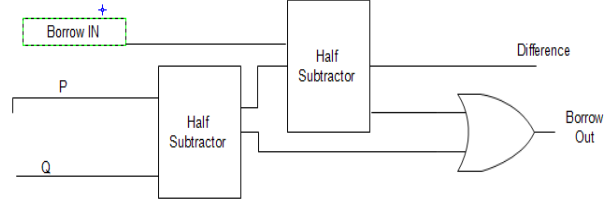
\includegraphics[width=0.75\columnwidth]{q2} % Example image
\end{center}
}
\end{homeworkProblem}

%----------------------------------------------------------------------------------------
%	PROBLEM 1
%----------------------------------------------------------------------------------------

% To have just one problem per page, simply put a \clearpage after each problem
\begin{homeworkProblem}
\textbf{Design full adder with only two 2-input X-OR and three 2- input NAND gates.}  \vspace{10pt} % Question

\problemAnswer{ 

Following is the implementation of a full adder using only two 2 input X- OR and three 2 input NAND gates. 
\begin{center}
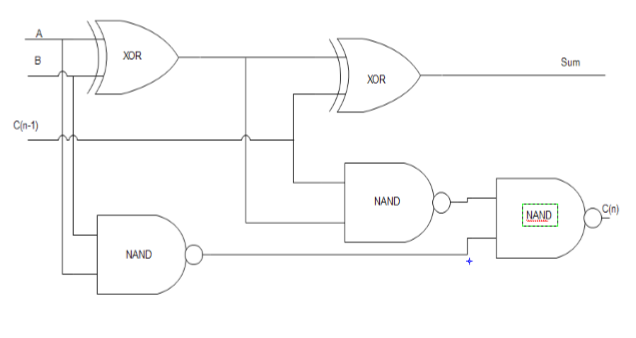
\includegraphics[width=0.75\columnwidth]{q3} % Example image
\end{center}
}
\end{homeworkProblem}


%----------------------------------------------------------------------------------------
%	PROBLEM 1
%----------------------------------------------------------------------------------------

% To have just one problem per page, simply put a \clearpage after each problem
\clearpage
\begin{homeworkProblem}
\textbf{Draw logic diagram for 4 bit gray code to binary converter.}  \vspace{10pt} % Question

\problemAnswer{ 
Following is the implementation of a gray code to binary converter.\\~\\
Binary Code : B$_{n-1}$ ...... B$_{0}$  \\~\\
Gray Code 	: G$_{n-1}$ ...... G$_{0}$ \\~\\
G$_{n-1}$ = B$_{n-1}$ and G$_{i}$ = B$_{i+1}$ XOR B$_{i}$ 
\begin{center}
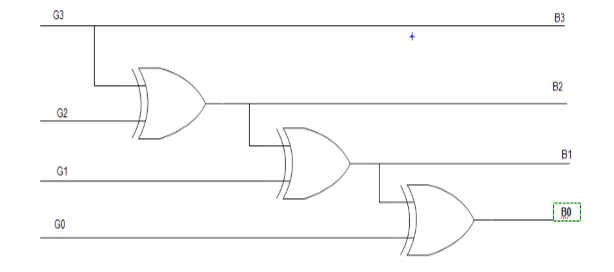
\includegraphics[width=0.75\columnwidth]{q4} % Example image
\end{center}
}
\end{homeworkProblem}
\end{document}
